% Created 2021-07-08 Thu 14:02
% Intended LaTeX compiler: pdflatex
\documentclass[presentation,mathserif,table]{beamer}
\usepackage[utf8]{inputenc}
\usepackage[T1]{fontenc}
\usepackage{graphicx}
\usepackage{grffile}
\usepackage{longtable}
\usepackage{wrapfig}
\usepackage{rotating}
\usepackage[normalem]{ulem}
\usepackage{amsmath}
\usepackage{textcomp}
\usepackage{amssymb}
\usepackage{capt-of}
\usepackage{hyperref}
\beamertemplatenavigationsymbolsempty
\usepackage[T1]{fontenc}
\usepackage{DejaVuSans}
\usefonttheme{professionalfonts}
\usepackage[euler-digits,euler-hat-accent]{eulervm}
\setbeamertemplate{itemize items}{•}
\setbeamertemplate{enumerate items}[default]
\setbeamertemplate{headline}{}
\setbeamertemplate{footline}{
\leavevmode%
\hbox{%
\begin{beamercolorbox}[wd=\paperwidth,ht=2.25ex,dp=1ex,right]{fg=black}%
\usebeamerfont{section in head/foot}\insertsection\hspace*{2em}
\insertframenumber{} / \inserttotalframenumber\hspace*{2ex}
\end{beamercolorbox}%
}%
\vskip0pt%
}
\usepackage{appendixnumberbeamer}
\setbeamersize{text margin left=3mm,text margin right=3mm}
\newcommand\blfootnote[1]{%
\begingroup
\renewcommand\thefootnote{}\footnote{#1}%
\addtocounter{footnote}{-1}%
\endgroup
}
\setbeamerfont{footnote}{size=\tiny}
\usepackage{tikz}
\usepackage[retainorgcmds]{IEEEtrantools}
\hypersetup{colorlinks=true, allcolors=., urlcolor=blue}
\usepackage[absolute,overlay]{textpos}
\newcommand{\eg}{e.g.\,}
\newcommand{\ie}{i.e.\,}
\newcommand{\aka}{a.k.a.\,}
\newcommand{\etc}{\emph{etc.}\,}
\newcommand{\X}{{\mathbold X}}
\newcommand{\x}{{\mathbold x}}
\newcommand{\Y}{{\mathbold Y}}
\newcommand{\y}{{\mathbold y}}
\newcommand{\B}{{\mathbold B}}
\newcommand{\R}{\mathbb{R}}
\DeclareMathOperator*{\argmin}{argmin}
\DeclareMathOperator*{\argmax}{argmax}
\DeclareMathOperator*{\tv}{TV}
\DeclareMathOperator*{\Tr}{Tr}
\DeclareMathOperator*{\FFT}{FFT}
\DeclareMathOperator*{\IFFT}{IFFT}
\DeclareMathOperator*{\diag}{diag}
\DeclareMathOperator*{\supp}{supp}
\DeclareMathOperator*{\tf}{tf}
\DeclareMathOperator*{\idf}{idf}
\DeclareMathOperator*{\df}{df}
\DeclareMathOperator*{\Var}{Var}
\DeclareMathOperator*{\Frob}{Frob}
\DeclareMathOperator*{\F}{F}
\DeclareMathOperator*{\softmax}{softmax}
\DeclareMathOperator*{\AUC}{AUC}
\usepackage{bm}
\usecolortheme{dove}
\setbeamercolor*{block title example}{fg=black,bg=white}
\setbeamercolor*{block body example}{fg=black,bg=white}
\usetheme{default}
\author{Jerome Dockes}
\date{}
\title{Machine learning Part 2}
\author{Jérôme Dockès}
\titlegraphic{
\includegraphics[height=1.5cm]{figures/mcgill-university.png} \hspace{1.5cm} 
\includegraphics[height=1.5cm]{figures/origami-lab-logo.png}}
\date{QLS course 2021-07-30}
\hypersetup{
 pdfauthor={Jerome Dockes},
 pdftitle={Machine learning Part 2},
 pdfkeywords={},
 pdfsubject={},
 pdfcreator={Emacs 26.3 (Org mode 9.3.7)}, 
 pdflang={English}}
\begin{document}

\maketitle
\section{Intro}
\label{sec:org1826700}
\subsection{Recap of part 1}
\label{sec:orgbc87aa9}
\begin{frame}[label={sec:org282e4bd}]{Recap of part 1}
\begin{block}{Supervised learning}
\begin{itemize}
\item Regression: least-squares linear regression
\item Classification: logistic regression
\end{itemize}
\end{block}
\begin{block}{Regularization}
\begin{itemize}
\item \(\ell_2\) \aka ridge regularization
\end{itemize}
\end{block}
\begin{block}{Model evaluation and selection}
\begin{itemize}
\item Out-of-sample generalization; independent test set
\item Performance metrics:
\begin{itemize}
\item regression: mean squared error
\item classification: accuracy, ROC curve
\end{itemize}
\item Cross-validation
\end{itemize}
\end{block}
\begin{structureenv} %% part1
Don't remember? watch Part 1 again!
\end{structureenv}
\end{frame}
\begin{frame}[label={sec:org066fb53}]{Notation \& vocabulary}
\begin{block}{Supervised learning framework}
\begin{equation}
Y = f(X) + E
\end{equation}
\vspace{-10pt}
\begin{itemize}
\item \(Y \in \R\): output (\aka target, dependent variable) to predict
\item \(X \in \R^p\): features (\aka inputs, regressors, descriptors, independent variables)
\item \(E \in \R\): unmodelled noise
\item \(f\): the function we try to approximate
\end{itemize}
\end{block}
\begin{block}{Example: linear regression}
\vspace{-20pt}
 \begin{IEEEeqnarray}{rCl}
 Y & = & \beta_0 + \langle X, \beta \rangle + E \\
& = & \beta_0 + \sum_{j=1}^p X_j \, \beta_j + E
 \end{IEEEeqnarray}
"learning" = estimating \(\beta_0 \in \R\) and \(\beta \in \R^p\)
\end{block}
\end{frame}
\section{Dimensionality reduction}
\label{sec:orga65990e}
\subsection{Intro}
\label{sec:org5d6af94}
\begin{frame}[label={sec:orgf8a02ab}]{Dimensionality reduction}
\begin{block}{Problems when the number of features \(p\) becomes large}
\begin{itemize}
\item Bigger errors on test data (larger variance of predictions)
\item Numerical stability issues
\item Computational cost and memory usage
\end{itemize}
\end{block}
\end{frame}
\begin{frame}[label={sec:org0ea6c72}]{Model complexity: overfitting}
\begin{itemize}
\item Model complexity increases with dimension.
\item Example: a linear model in dimension \(p\) can fit exactly (0 training error) any set of \(p + 1\) points.
\item Risk of overfitting: fitting exactly training data but failing on test data
\end{itemize}

\begin{center}
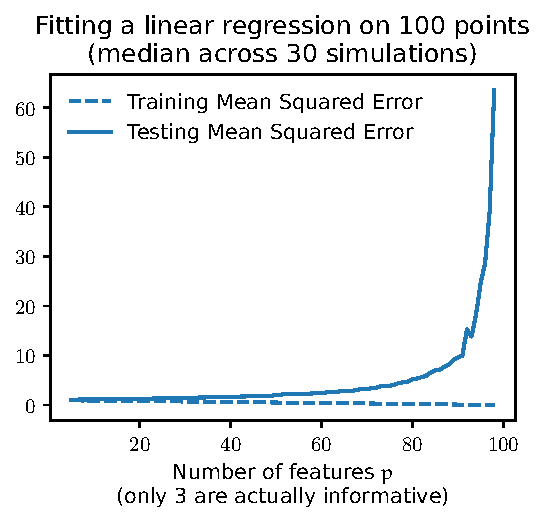
\includegraphics[height=.7\textheight]{figures/generated/ridge_overfitting/mse.pdf}
\end{center}
\end{frame}
\begin{frame}[label={sec:org4b43f06}]{Cost of fitting many parameters}
\begin{itemize}
\item Many algorithms require polynomial time in \(p\)
\item Implementations often make copies of the design matrix (\eg for centering \& rescaling)
\end{itemize}
\begin{center}
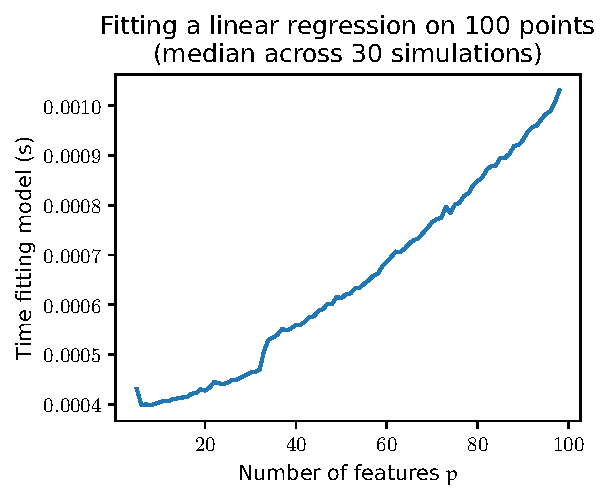
\includegraphics[height=.7\textheight]{figures/generated/ridge_overfitting/durations.pdf}
\end{center}
\end{frame}
\subsection{Univariate feature selection}
\label{sec:orgb1e48ea}
\begin{frame}[label={sec:org7d5aa73}]{Univariate feature selection}
\begin{itemize}
\item \aka feature screening, filtering \ldots{}
\item Check features (columns of \(X\)) one by one for association with the output \(y\)
\item Keep only a fixed number or percentage of the features
\end{itemize}
\begin{block}{Simple (linear) association criteria}
\begin{itemize}
\item for regression: correlation
\item for classification: ANalysis Of VAriance
\end{itemize}
\end{block}
\begin{block}{Read more in the scikit-learn user guide}
\url{https://scikit-learn.org/stable/modules/feature\_selection.html\#feature-selection}
\end{block}
\end{frame}

\begin{frame}[label={sec:orge8dbcce}]{Univariate feature selection}
Keeping only the 10 best features (most correlated with \(y\))
\begin{center}
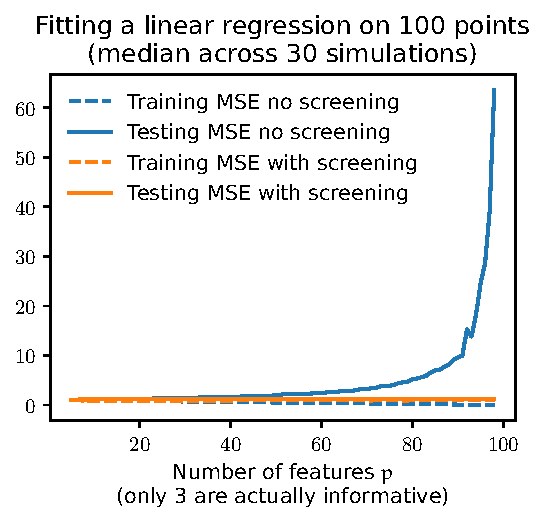
\includegraphics[height=.7\textheight]{figures/generated/ridge_overfitting/mse_with_dim_reduction.pdf}
\end{center}
\end{frame}

\begin{frame}[label={sec:org2d8934d}]{Same plot in log scale}
\begin{center}
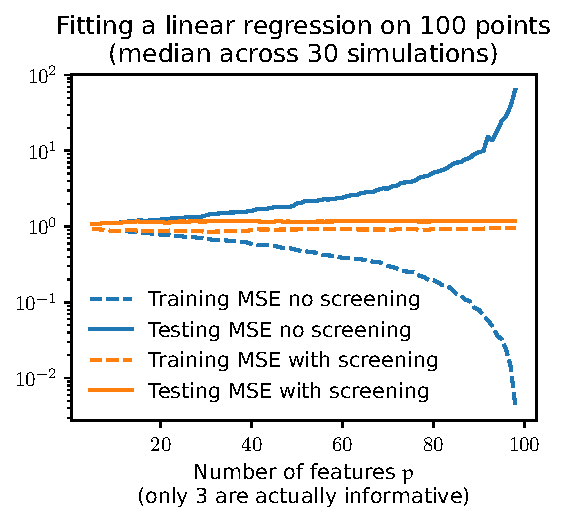
\includegraphics[height=.7\textheight]{figures/generated/ridge_overfitting/mse_with_dim_reduction_log.pdf}
\end{center}
\end{frame}

\subsection{Linear decomposition methods}
\label{sec:org5658fcc}
\begin{frame}[label={sec:orgbc12549}]{Linear decomposition methods}
\begin{block}{Maybe OK to drop \(X_2\):}
\vspace{-10pt}
\begin{center}
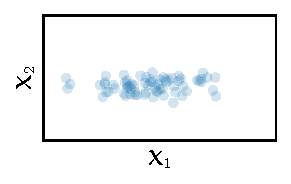
\includegraphics[height=.3\textheight]{figures/generated/pca/cloud_aligned.pdf}
\end{center}
\vspace{-20pt}
\end{block}
\begin{block}{Data low-dimensional but no feature can be dropped:}
\begin{center}
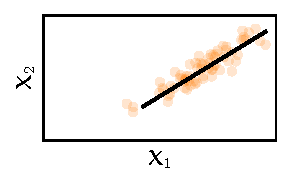
\includegraphics[height=.3\textheight]{figures/generated/pca/cloud_not_aligned.pdf}
\end{center}

Find a better referential in which to represent the data
\end{block}
\end{frame}
\begin{frame}[label={sec:org0c683d0}]{Linear regression: projection on the column space of \(X\)}
\begin{block}{Approximate \(y\) as a combination of the columns of \(X\)}
\begin{equation}
\hat{\y} = \X \, \hat{\beta} \in \R^n
\end{equation}
\begin{itemize}
\item The columns of \(X\) are a family of \(p\) \(n\)-dimensional vectors
\item When \(p\) is high or the columns of \(X\) are correlated, we want to use a family of \(k < p\) instead
\item Feature selection: drop some columns, keep only \(k\)
\item Could we build a better family of \(k\) vectors?
\end{itemize}
\end{block}
\end{frame}

\begin{frame}[label={sec:org8522074}]{Principal Components Regression}
\begin{itemize}
\item Approximation of \(X\) of rank \(k\): find a family of \(k\) basis vectors and approximate each column of \(X\) as a mixture of these \(k\) vectors
\item Find the family that gives the best approximation: the one with the smallest Frobenius norm of the reconstruction error.
\item This is the same as finding the \(k\) orthogonal directions in which \(X\) varies the most
\end{itemize}
\end{frame}

\begin{frame}[label={sec:orgbeb0771}]{Principal Components: feature space}
\begin{center}
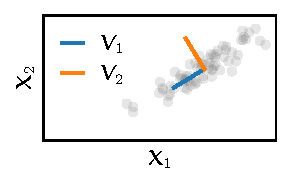
\includegraphics[height=.3\textheight]{figures/generated/pca/cloud_not_aligned_with_pc.pdf}
\end{center}
\end{frame}

\begin{frame}[label={sec:org31fc2e9}]{Ridge regression and PCA}
\begin{itemize}
\item Both ridge regression and PC regression compute the coordinates of \(y\) in the basis given by the SVD of \(X\)
\item ridge shrinks the coefficients of sv \(d_j\) by a factor \(d_j^2 / (d_j^2 + \lambda)\)
\item PC regression sets the coefficient to 0 for all but the \(k\) largest \(d_j\)
\end{itemize}
\end{frame}
\begin{frame}[label={sec:org9abd636}]{Other decomposition methods}
\begin{itemize}
\item Take \(y\) into account
\item Different criteria (sparsity, independence, \ldots{})
\end{itemize}
\end{frame}

\section{More on cross-validation}
\label{sec:orge27c722}
\subsection{More on cross-validation}
\label{sec:org14da6f6}


\begin{frame}[label={sec:org611dcc4}]{Nested cross-validation: setting hyperparameters}
\begin{block}{How can we choose:}
\begin{itemize}
\item Number of features or PCA components \(k\)?
\item The ridge hyperparameter \(\lambda\)?
\end{itemize}

Try a few and pick the best one\ldots{}
But measure its performance on separate data!
\end{block}
\end{frame}
\begin{frame}[label={sec:org4d642ae}]{Some common pitfalls with cross-validation}
\begin{itemize}
\item Ignoring dependencies between samples
\item Ignoring dependencies between CV scores
\item Over-interpreting good CV scores
\end{itemize}
\end{frame}

\begin{frame}[label={sec:org1aa26ac}]{Two sources of variance: training data and test sample}
Don't use Leave-One-Out Cross-validation
\end{frame}
\section{Neuroimaging application: a task-fMRI decoding pipeline}
\label{sec:orgd5c9ab5}
\subsection{FMRI decoding}
\label{sec:orge90a6ce}
\begin{frame}[label={sec:orgf494b0a}]{fMRI decoding}
\begin{itemize}
\item Describe data and task
\end{itemize}
\end{frame}
\begin{frame}[label={sec:org23976d8}]{The decoding pipeline}
\begin{itemize}
\item Masking: extracting voxels that are inside the brain
\item Feature selection with ANOVA
\item Classifier: logistic regression
\end{itemize}
\end{frame}
\begin{frame}[label={sec:org36585a5}]{Implementation: in class}
\end{frame}
\end{document}